\section{Trabalho Previamente Desenvolvido}
O trabalho elaborado por \citeonline{RUANI} tinha como objetivo geral: Desenvolver um dispositivo do tipo luva sensora capaz de 
reconhecer configurações de mão, correspondente ao alfabeto manual de LIBRAS, e realizar a tradução destas para o seu significado 
na Língua Portuguesa, apresentando o resultado na forma de texto em um \textit{display}. A luva foi desenvolvida a partir de sensores indutivos, incluindo circuito de excitação
para as bobinas, assim como circuito de leitura e sistema embarcado usando o 
microcontrolador MSP430F5529.

\subsection{Construção das bobinas}
Com base no trabalho de \citeonline{baseadoruani}, foi possível obter um método para construir uma luva com sensores indutivos 
que tem o funcionamento explicado na seção \ref{sec:indutivo}. 	
Para obter a posição dos sensores na luva foi observado diferentes sinais de LIBRAS e como eles se diferem, por exemplo U e V, 
somente o ângulo entre o dedo indicador e dedo médio pode diferenciar essas letras. Considerando todas as letras e suas posições 
de mão, foi obtido o seguinte esquema de sensores e geradores, como demonstrado na Figura \ref{fig:disposicaoSensores}.

	\begin{figure}[H]
		\vspace{4mm}
		\centering
		\caption{Mapa de sensores e geradores de sinal na luva}
		\label{fig:disposicaoSensores}
		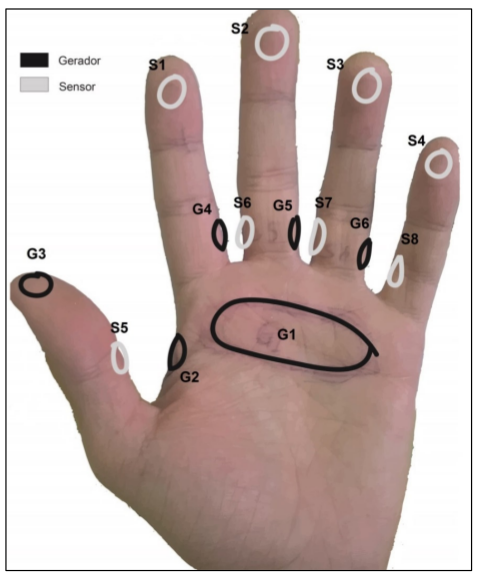
\includegraphics[scale=0.5]{imagens/SensoresMao.png}		
		\caption*{Fonte: \citeonline[p. 68]{RUANI}.}		
	\end{figure}
	
	
A espessura das bobinas foi definida para que não atrapalhasse no movimento normal da mão ao vestir a luva, tendo $14\textrm{ }mm$ de 
diâmetro. Todas as bobinas foram construídas a mão e com o mesmo número de espiras. Naturalmente que devido ao processo manual de 
fabricação há uma variação nas indutâncias. A frequência ressonante  do circuito LC foi definida em torno de $100\textrm{ }kHz$, 
projetando o 
resto dos componentes a partir disso. Uma das bobinas construídas é exibida na Figura \ref{fig:bobinas}.


	\begin{figure}[H]
		\vspace{4mm}
		\centering
		\caption{Bobina construída para luva}
		\label{fig:bobinas}
		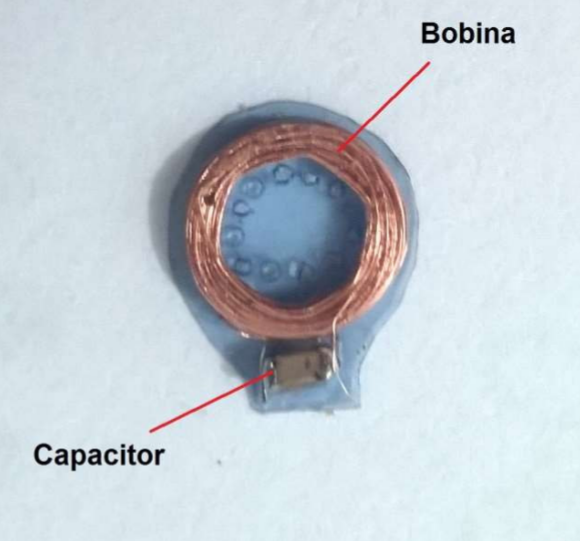
\includegraphics[scale=0.25]{imagens/SensorIndutivo.png}
		\caption*{Fonte: \citeonline[p. 71]{RUANI}.}		
	\end{figure}

 O resultado é apresentado na Figura \ref{fig:luvaRuani}, onde é mostrada a luva construída com os sensores indutivos.

	\begin{figure}[H]
		\vspace{4mm}
		\centering
		\caption{Vista frontal e lateral da luva sensora desenvolvida}
		\label{fig:luvaRuani}
		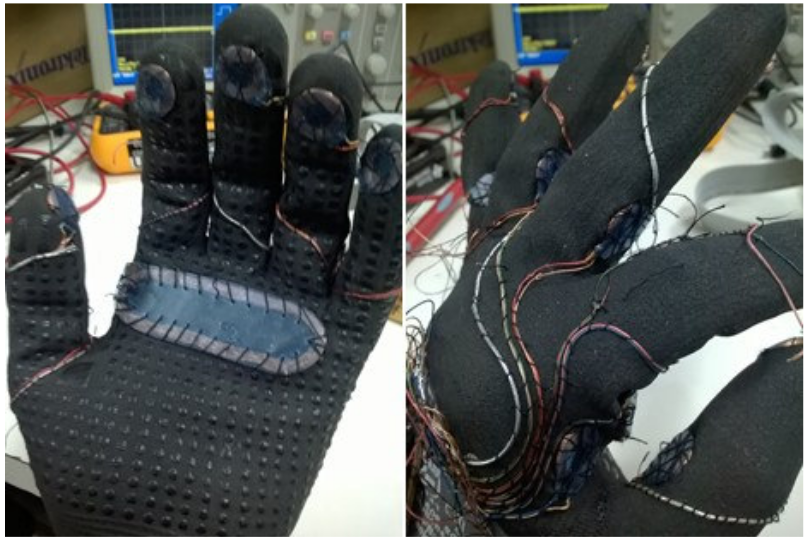
\includegraphics[scale=0.5]{imagens/luvaRuani.png}	
		\caption*{Fonte: \citeonline[p. 87]{RUANI}.}		
	\end{figure}

	

\subsection{Circuito de condicionamento de sinais}
\label{sec:placa}
Para o funcionamento do sistema como um todo, todos os sinais provenientes dos sensores indutivos devem ser tratados para a  
leitura correta no conversor analógico digital (ADC) do microcontrolador.
Na figura \ref{fig:hard} é possível ver todo o tratamento de \textit{hardware} feito para o processamento dos sinais do sensores 
indutivos.

\begin{figure}[H]
	\vspace{4mm}
  	\centering
	\caption{Diagrama de blocos do sistema desenvolvido por \citeonline[p.65]{RUANI}}		
  	\label{fig:hard}	
  	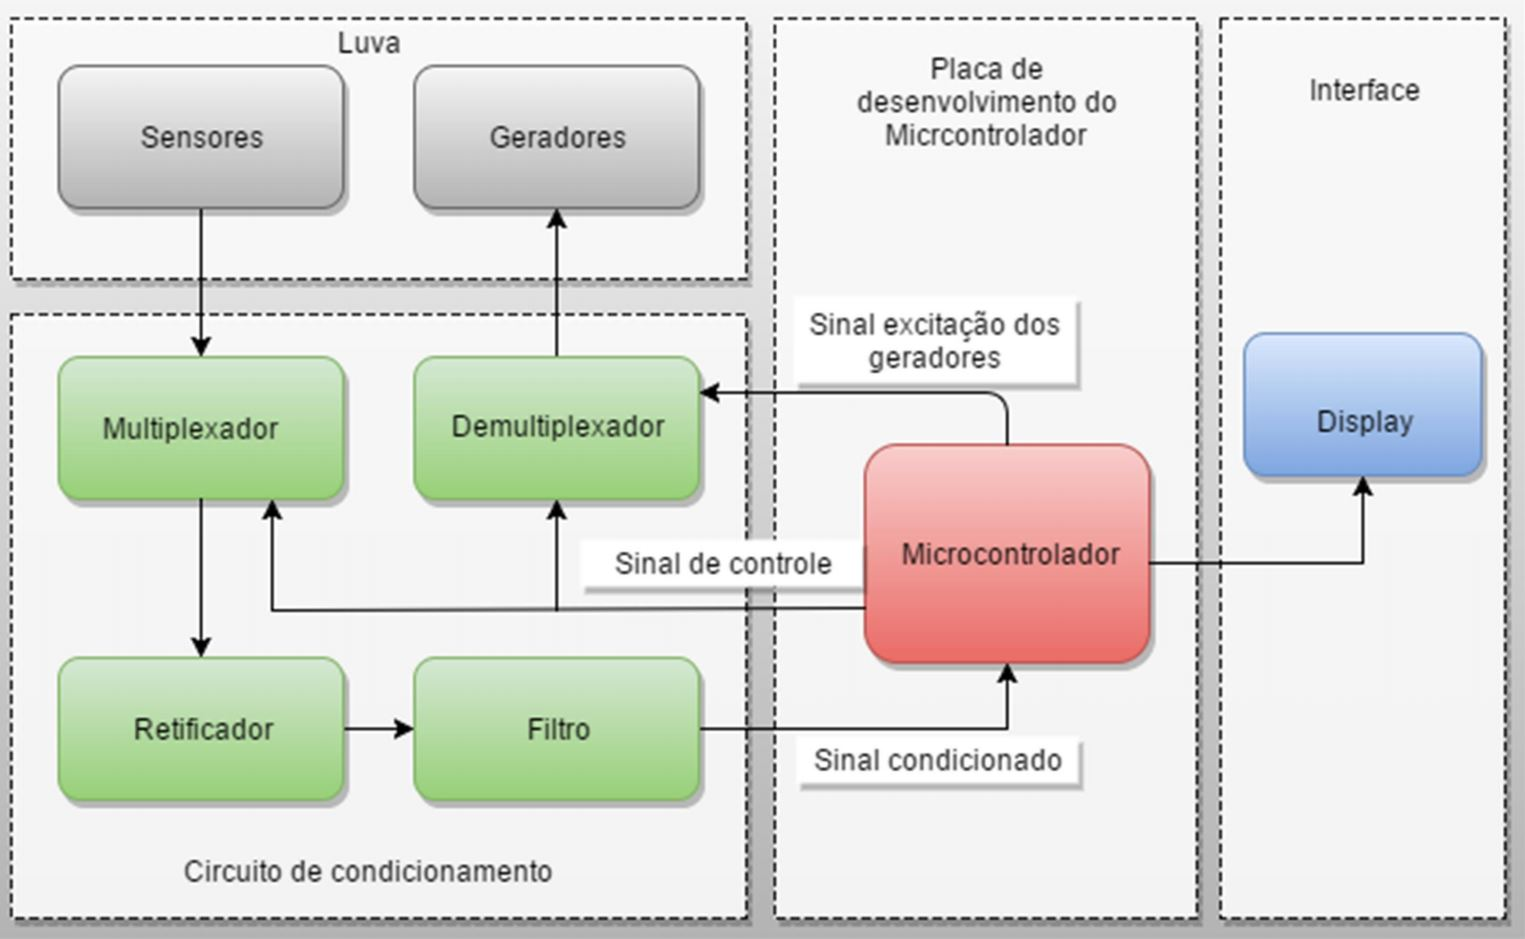
\includegraphics[scale=0.3]{imagens/desc_luva_ruani.JPG}
  	\caption*{Fonte: \citeonline[p. 65]{RUANI}.}
\end{figure}

A modelagem do circuito de aquisição e processamento dos sinais foi proposta por \citeonline{baseadoruani}, o qual 
foi adaptado para simplificar o circuito. Uma das modificações foi substituir o gerador senoidal e deixar o microcontrolador 
gerar uma onda quadrada, considerando que a mudança de forma de onda não interfere significativamente na resposta dos sensores, 
sendo que é a frequência que determina a ressonância dos geradores \cite{RUANI}.

Um circuito retificador a envoltória do sinal CC é necessário para converter um sinal CA em um sinal CC. Para que a saída represente o pico do sinal CC, 
é necessário empregar um detector de pico seguido de um filtro passa-baixas \cite{Boylestad}.

De acordo com \cite{malvinaodamassa}, um filtro permite a passagem de uma faixa de frequências enquanto rejeita outra. Filtros 
podem separar os sinais desejados dos indesejados, bloquear sinais de interferência e modificar sinais. Existem os filtros 
passivos que são constituídos de resistores, capacitores e indutores. Também existem os ativos, que são compostos de resistores, 
capacitores e amplificadores operacionais ou amp-ops.

O uso de amp-ops nos filtros ativos pode eliminar a necessidade dos volumosos indutores, que não são satisfatórios quando 
integrados aos circuítos. Em contrapartida, filtros ativos não atenuam necessariamente os sinais sobre a banda passante, como acontece 
com seus similares feitos com elementos passivos \cite{Cathey}.

Como são utilizadas várias bobinas, utiliza-se de uma técnica para não ter leituras afetadas por interferência, utilizando o 
método de divisão de tempo, onde cada bobina geradora é acionada sozinha por um período de tempo. O sinal de saída do 
multiplexador deve passar por um processo de condicionamento, primeiramente por um atenuador, para que o valor de amplitude se
fique adequado ao valor de alimentação dos amplificadores operacionais \cite{RUANI}.

Em seguida, o sinal passa por um circuito retificador, uma vez que a informação que possibilita estimar a posição das bobinas é 
o modulo da fem induzida nas bobinas dos sensores. O sinal retificado é filtrado para eliminar \textit{ripple} do sinal, e em 
seguida passa por ajustes de amplitude para ser conectado ao ADC do microcontrolador.
	

	
	
	
	
	
	